\chapter {NOTION DE BASE SUR L’OPTIMISATION.}     % numéroté chap 1
\thispagestyle{fancy}
\definecolor{blue}{RGB}{51,131,255}
%\includegraphics{images/logo_3IAC} 
%
%\section{c'est quoi la gestion des sinistres?}

%Prévoir l'avenir et tenter de savoir si telle de nos actions futures nous sera %favorable, ce que l'on peut réaliser avec des chances de succès ou ce que l'on %doit éviter d'entreprendre est le souci de chaque être humain. C'est une %préoccupation qui n'échappait pas aux hommes de l'Antiquité. Les devins %répondaient à leurs attentes en examinant notamment le vol des oiseaux. Le fait, %d'en apercevoir un, perché ou volant à gauche, en latin "sinister", était un signe %jugé défavorable. En vieux français, ce mot latin avait donné "senestre".

%De nos jours, le mot est utilisé dans le vocabulaire juridique du droit des assurances, pour désigner toutes circonstances prévues au contrat d'assurance comme, le vol, l'incendie, le décès du souscripteur ou d'un tiers, un naufrage, ou un dégâts des eaux, dont la survenance génère pour la compagnie d'assurances l'obligation d'exécuter la prestation convenue.[Code des assurances, Articles L112-1]%

\section{En préalable à l’optimisation des processus }
	\subsection{Qu’est-ce qu’un processus.}
 Un processus \cite{Ref20} est un ensemble d'opérations ou d'activités réalisées par des acteurs avec des moyens et selon des références en vue d'une finalité. Dans le cadre des démarches qualité, un processus doit toujours être tourné vers un bénéficiaire ou un système bénéficiaire, interne ou externe.
Un processus peut comprendre des activités réalisées par différents services, différentes entités. Ce caractère transversal, supposant de nombreuses interfaces, est souvent un des points cruciaux de l'amélioration du service ou du produit fourni aux bénéficiaires. 

	\subsection{Pourquoi les optimiser ?\cite{Ref21}}
Une action sur les processus vise différents objectifs : 

\begin{itemize}[label=\textbullet, font=\LARGE \color{blue}]
	\item mieux prendre en compte les attentes des bénéficiaires pour améliorer les services fournis 
	\item permettre aux différents acteurs de s'impliquer dans le fonctionnement du processus,
	\item clarifier les rôles et responsabilités des acteurs, définir les marges de manœuvre et les cohérences nécessaires, simplifier les interfaces entre entités ; 
	\item transformer ou créer un nouveau processus pour répondre à de nouvelles attentes ;
	\item diminuer les coûts, les délais d'un processus, augmenter sa performance au regard d'indicateurs définis ; 
	\item mieux réagir aux aléas ; 
	\item viser une certification via la mise en place d'un système qualité ;
	\item accompagner la mise en place d'un progiciel de gestion… 
\end{itemize} 
	\subsection{A quel moment faut-il le faire ?}
Le travail sur les processus s'inscrit en général dans le cadre d'une démarche qualité. Cette démarche doit par conséquent être lancée : affichage de la politique qualité\cite{Ref9} et de ses axes, communication aux personnels, engagement de la direction, plan d'action, formation des acteurs clés.
Par ailleurs, l'optimisation des processus est une méthode qui accompagne efficacement différents types de démarches : 

\begin{itemize}[label=\textbullet, font=\LARGE \color{blue}]
	\item Des démarches qualité comme, par exemple, l’élaboration d’engagements de service, la certification selon les normes ISO, la réduction de dysfonctionnements 
	\item Mais aussi d’autres démarches comme, par exemple, les réorganisations globales, les fusion de service, la gestion des compétences, l’émergence de nouvelles activités.
\end{itemize} 

\section{Les principes de base de l’optimisation des processus}
\subsection{Bien caractériser le périmètre couvert par le processus}

L'essoufflement des démarches d'optimisation des processus s'explique bien souvent par un mauvais cadrage du périmètre des différents processus. Ces zones de flous provoquent vite des débats, des revendications des pilotes des différents processus. Il convient donc de définir avec précision les champs que couvre chaque processus, en terme d'activités, de productions mais aussi d'acteurs. Cette tâche se révèle parfois difficile lorsque les processus sont transverses à différentes entités. 
\subsection{Identifier les interfaces }
C'est souvent aux interfaces entre processus ou entre entités à l'intérieur d'un même processus que se situent les principales zones d'amélioration potentielle. Il convient donc de les identifier au mieux, d'un point de vue commun aux différents acteurs qui y interviennent. Il est également important d'étudier, à ces interfaces, les modalités de circulation de l'information liée au processus : y-a-t-il une bonne traçabilité ? Les informations importantes des étapes passées sont-elles bien prises en compte aux étapes suivantes ? N'y-a-t-il pas de jeux d'acteurs aux interfaces avec des objectifs de pouvoir par rétention d'informations ?
\subsection{Ne travailler que des processus-clés ou processus critiques  }
Le travail sur les processus doit être cadré d'un point de vue stratégique et ne viser qu'à améliorer des performances qui font sens au niveau du service et de ses bénéficiaires. Il ne s'agit donc pas de travailler sur l'ensemble des processus, mais seulement sur quelques-uns qui pourraient apparaître prioritaires au vu de différents critères : 
\begin{itemize}[label=\textbullet, font=\LARGE \color{blue}]
	\item Forts dysfonctionnements,
	\item Insatisfaction des bénéficiaires ou émergence de nouvelles attentes,
	\item Évolution de la stratégie du service
\end{itemize}
 \subsection{Privilégier une approche participative  }
 Les démarches d'optimisation de processus les plus efficaces sont celles qui associent assez étroitement les acteurs des processus dans leur amélioration. A charge du pilote de fixer les modalités de ce travail participatif, en les échelonnant dans le temps. Une discussion sur la caractérisation du processus est, dans tous les cas, indispensable. Les travaux peuvent également associer des bénéficiaires. Enfin, il est important, sur ces processus-clés, d'anticiper les possibles résistances au changement des acteurs face aux évolutions : optimiser un processus signifie souvent modifier des pratiques routinières et davantage se tourner vers les bénéficiaires.
 \subsection{Garder de la souplesse dans la formalisation pour rester ouvert à l’urgence  }
 La formalisation des processus ne doit pas créer un système rigide dans lequel chaque acteur se limiterait à observer à la lettre la procédure. Au contraire, ce système doit être ouvert, pour permettre et même favoriser les initiatives des acteurs, et adaptable, pour pouvoir réagir aux aléas, aux urgences, et à plus long terme aux évolutions des attentes des bénéficiaires. Dans certains cas, il peut même être utile de configurer un processus spécifique, adapté, pour traiter au mieux l'urgence. 
Il faut enfin noter que le degré de formalisation d'un processus varie selon les compétences des acteurs qui le font fonctionner. De façon générale, plus les compétences sont élevées, moins la formalisation est stricte. Elle est alors remplacée par la maîtrise professionnelle des acteurs.


%En tant qu’agent générale d’ACTIVA, PRIMA Assurances évolue dans le monde du %marché des assurances Camerounais qui est de plus en plus complexe. Connecté au %travers de multiples réseaux et dans lequel tous les acteurs ont de nouvelles %exigences, contraintes et face aux vulnérabilités générées par ces mutations, %PRIMA Assurances s’adapte pour mieux protéger ses actifs, qu’ils soient %matériels ou immatériels, sa marque, son image ou sa réputation, mais aussi la %qualité de ses femmes et de ses hommes afin de parfaire sa stratégie, son %organisation, sa capacité à innover ou son savoir-faire.

\section{Une démarche possible pour optimiser un processus\cite{Ref11}}

Nous proposons une démarche en plusieurs étapes séquencées. Selon le contexte, la stratégie, les priorités de votre service, des poids différents peuvent être mis derrière ces étapes. Nous conseillons dans tous les cas de mettre au point la démarche de façon précise, par exemple en suivant les principes de la conduite de projet. Cela suppose notamment de bien cadrer la démarche ou le projet d'optimisation, de nommer un pilote pour chaque processus, de définir un dispositif de suivi, de formaliser un calendrier et d'allouer les moyens nécessaires. 
 \subsection{Cartographier les processus  }
Pour aborder une démarche globale de travail sur les processus, il est utile d'en avoir une vision d'ensemble. Un repérage de l'ensemble des grands processus d'une organisation peut ainsi être réalisé sous la forme d'un schéma. Les conventions suivantes peuvent être respectées : 
\begin{figure}[H]
	\centering
	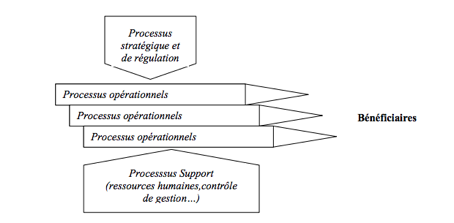
\includegraphics[width=13cm]{cartographie.png}
	\caption{Cartographie des processus}{ \begin{center} source : \textit{Groupe de travail - Optimisation des processus - Etienne Jasmin} \end{center}}
	\label{fig:CIMA}
\end{figure}

	\subsection{Choisir les processus-clés}	
	
A l'intérieur de la cartographie précédente, il ne s'agit pas toujours de vouloir optimiser tous les processus, sauf si l'on souhaite se réorganiser entièrement. Différents critères peuvent ainsi aider aux choix des processus sur lesquels les travaux d'optimisation porteront en priorité : 
\begin{itemize}[label=\textbullet, font=\LARGE \color{blue}]
	\item Constats des dysfonctionnements,
	\item Insatisfaction des bénéficiaires ou émergence de nouvelles attentes,
	\item Évolution de la stratégie ou émergence de nouvelles attentes,
	\item Développement de nouvelles démarches (ARTT, gestion des compétences) qui peuvent avoir un impact fort sur certains processus,
	\item Mise en place de nouveaux outils informatiques et notamment et progiciels de gestion intégrée,
	\item Lancement d’une démarche d’engagements de service (pour s’engager vis à vis d’un bénéficiaires, il est impératif de maîtriser les processus afférents)
\end{itemize}
	
    \subsection{Caractériser un processus } 
	
Il s’agit de répondre aux questions suivantes :
\begin{itemize}[label=\textbullet, font=\LARGE \color{blue}]
	\item Quelle est la finalité du processus ?
	\item Quel est le bénéficiaire ou le système bénéficiaire du processus ?
	\item Quel(s) est(sont) le(s) service(s) ou produit(s) fourni(s) ?
	\item Quelles sont les exigences des bénéficiaires par rapport à ce service / produit ?
	\item Quels sont les indicateurs qui permettent de mesurer le respect de ces exigences et plus globalement la performance du processus ?
	\item Quels sont les acteurs qui concourent directement au processus ?
	\item Quels sont les principaux moyens utilisés ?
	\item Quels sont les éléments d’entrée du processus ? (ce sont parfois les éléments déclencheurs) ?
	\item Quels sont les fournisseurs de ces éléments ?
	\item Quelles sont les exigences du processus par rapport à ces fournisseurs ?
	\item Quels sont les indicateurs qui permettent de mesurer le respect de ces exigences ?
\end{itemize}

Le repérage des exigences des bénéficiaires est une étape cruciale de la caractérisation du processus. Elle peut mériter une enquête approfondie auprès des bénéficiaires.

Enfin, lorsque la démarche porte sur plusieurs processus, il est important, à partir de leurs caractérisations, de vérifier qu’ils ne se recouvrent pas ou alors que leurs interfaces sont clairement identifiées.


	\subsection{Décrire un processus }
	
Il s’agit de réaliser une description d’ensemble du processus avec la présentation synthétique des activités et de leurs responsables. Ce travail peut utilement se faire sous la forme d’un diagramme « qui fait quoi ». Les principales étapes du processus peuvent ensuite être identifiées, les principaux points de contrôle et les indicateurs actuels également. Cette représentation synthétique du processus permet d'en prendre connaissance rapidement et de susciter de façon participative des interrogations sur l'enchaînement des activités, les relations entre acteurs et avec les bénéficiaires. 


	\subsection{Diagnostiquer un processus et son contexte pour définir les objectifs d’optimisation}

A partir de la description précédente, il s'agit de mener un diagnostic approfondi du processus. Ce diagnostic repose sur l'identification précise des principaux faits marquant le fonctionnement du processus et son contexte. Ces faits peuvent par exemple porter sur : 

\begin{itemize}[label=\textbullet, font=\LARGE \color{blue}]
	\item Les dysfonctionnements internes au processus, 
	
	\item Les non-qualités constatées, 
	
	\item La fréquence des anomalies, 
	
	\item Les insatisfactions des bénéficiaires, 
	
	\item Les évolutions des indicateurs (coût, délai…), 
	
	\item Les temps passés à la réalisation de tout ou partie du processus,  
	
	\item L'émergence de nouvelles attentes des bénéficiaires
\end{itemize}

Une fois le diagnostic réalisé, il s'agit de le traduire sous forme d'objectifs clairement formulés et visant l'optimisation du processus : "réduire de 15\% le temps passé à l'accomplissement de cette partie de processus", "accélérer d'un jour les délais", "réduire le nombre d'anomalies de 20\%", "augmenter de 2 points la satisfaction des bénéficiaires".

\subsection{Choisir le degré d’optimisation : améliorer ou reconcevoir selon des objectifs et indicateurs de performance}

En fonction des objectifs identifiés à partir du diagnostic précédent, il s’agit de décider des actions à mener. Celles-ci peuvent avoir une ampleur très variable, selon deux dimensions : 
\begin{figure}[H]
	\centering
	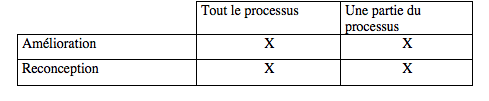
\includegraphics[width=13cm]{exmpleindicateur.png}
	\caption{Exemple d'indicateurs}{ \begin{center} source : \textit{Groupe de travail - Optimisation des processus - Etienne Jasmin} \end{center}}
	\label{fig:exemple d'indicateur}
\end{figure}

Une action d'amélioration consiste à reprendre le processus existant pour agir sur certains de ses facteurs. Exemples : mise en parallèle de certaines étapes, suppression d'une étape, changement d'outil sur une étape, développement des compétences pour une tâche, mise en place d'indicateurs à un point stratégique du processus, modification de la procédure régissant une activité.

Une action de reconception ne part pas du processus existant. Elle ne se base que sur les niveaux de performance visés et les moyens et ressources disponibles pour concevoir un tout nouveau processus, avec des façons de faire nouvelles, des enchaînements non encore pratiqués.

\subsection{Optimiser le processus}

En fonction des objectifs précédemment identifiés, il s'agit de décider des actions d'optimisation à mettre en œuvre, actions qui conduiront à modifier de façon plus ou moins forte le processus. Les modalités de ce travail varient en fonction des actions décidées. Quelques conseils restent néanmoins valables pour tout type d'optimisation : 

\begin{itemize}[label=\textbullet, font=\LARGE \color{blue}]
	\item Procéder d'abord sur papier en représentant le processus cible, 
	\item Faire réagir les acteurs concernés, 
	\item Procéder ensuite par tests successifs des différentes phases du processus, rectifier ce qui s'avère difficile à mettre en œuvre, 
	\item Concevoir les actions d'accompagnement à mettre en œuvre (formation, gestion des compétences, outillage…), 
	\item Communiquer tout au long de ces phases, 
	\item Installer enfin l'ensemble du processus, en permettant, sur un délai limité, les ajustements nécessaires à sa bonne mise en œuvre, 
	\item Installer l'ensemble des indicateurs : indicateurs sur le processus (en cours de production) et indicateurs de résultats (sur le produit / service fourni et sur la satisfaction des bénéficiaires), 
	\item Définir le pilote de processus (personne ou fonction)
\end{itemize}

\subsection{Mettre en œuvre et piloter le nouveau processus}

Une fois installé, le processus doit vivre sur le long terme. Son pilotage en continu est indispensable : 

\begin{itemize}[label=\textbullet, font=\LARGE \color{blue}]
	\item de façon opérationnelle : suivi des indicateurs de processus et de résultat, traitement des dysfonctionnement, relevé de fonctionnement, bouclages, traitement des suggestions des acteurs du processus, suivi des moyens mis en œuvre, suivi des compétences
	\item et de façon stratégique : réorientations du processus selon les évolutions du contexte, de l'environnement, des attentes, maintien de la cohérence entre le processus piloté et le système global. 
\end{itemize}